\label{mapeamento_sistematico}

Este capítulo descreve o mapeamento sistemático, método utilizado para estruturar a pesquisa da literatura. A pesquisa possibilita identificar, avaliar e interpretar outros trabalhos científicos, além de contribuir no estudo e na resposta da questão desta pesquisa, como afirma os autores Kitchenham \textit{et al.} \cite{kitchenham2007guidelines,petticrew2008systematic,de2018mapeamento}. O objetivo desta revisão é verificar na literatura textos correspondentes às questões definidas neste trabalho, e que possam colaborar nas respostas sobre monitoramento de sistemas distribuídos.

%%%%%%%%%%%%%%%%%%%%%%%%%%%%%%%%%%%%%%%%%%%%%%%%%%%%%%%%%%%%%%%%%%%%%%%%%%%%%%%

\section{Questões de Pesquisa}
\label{questoes1e2}

Para alcançar o objetivo, foram levantadas algumas questões de pesquisa \textbf{(QP)}, neste trabalho serão utilizadas 2 questões, com o intuito de fornecer auxílio na fundamentação da pesquisa relacionada ao monitoramento de sistemas distribuídos, as questões são descritas a seguir. As questões têm a intensão de fornecer subsídio durante a busca de informações sobre o tema possibilitando identificar trabalhos, e experiências técnicas que já foram executadas e analisadas, como Feltrim\cite{feltrim2004abordagem} descreve em seu trabalho.

\begin{description}
\item[QP1)] Quais os estudos primários existentes na literatura que discutem os mecanismos de monitoramento 
que são aplicados à sistemas distribuídos?
\item[QP2)] Quais são as principais características relativas ao monitoramento de sistemas
distribuídos mencionadas na literatura?
\end{description}

%%%%%%%%%%%%%%%%%%%%%%%%%%%%%%%%%%%%%%%%%%%%%%%%%%%%%%%%%%%%%%%%%%%%%%%%%%%%%%%%

\section{Estratégia de busca}
\label{sec:stringbusca}

Para identificação e busca dos trabalhos, com maior relevância e aderência ao tema abordado, e definido nas questões de pesquisa, foi criada uma \textit{string} de busca. De acordo com Keele \textit{et al.} \cite{keele2007guidelines}, a forma para criação de uma \textit{string} de busca, é feita a partir da identificação de sinônimos, abreviações. E também por meio de operadores lógicos, como por exemplo, \textit{AND} e \textit{OR} que auxiliam e permitem concatenar os termos identificados, o que possibilita a elaboração de uma \textit{string}. 

Para realização da pesquisa levou-se em conta os padrões e tecnologias mais comuns do mercado utilizados para o monitoramento de sistemas distribuídos, juntamente com algumas palavras-chave: \textit{"Monitoring Protocol"}, \textit{"Distributed Systems"}, \textit{"Monitoring"}, "\acrshort{SOA}", "\textit{web services}" e "\acrshort{ESB}". As palavras chave foram escritas em inglês, para uma maior abrangência de trabalhos publicados em jornais e revistas internacionais. Diante da situação obteve-se a seguinte \textit{string} de busca: \textit{(("Protocol Monitoring" OR "Monitoring Systems") AND ("Distributed Systems"OR "SOA")) OR ( ("ESB" AND "Web Services" AND "REST"))}.

De acordo com Kitchenham \cite{kitchenham2007guidelines}, a obtenção da \textit{string} de busca, foi iniciada a pesquisa dos trabalhos e artigos científicos, as pesquisas foram realizadas nas bases de dados digitais que indexam os principais trabalhos científicos do ramo da \acrlong{TI}, para essa atividade foi utilizado um protocolo de pesquisa para execução do mapeamento sistemático, o protocolo foi separado por etapas, uma representação protocolo de pesquisa poderá ser visualizada na figura \ref{fig:etapasRSL}, a execução das etapas proporcionaram uma maior abrangência no acesso à literatura do tema pesquisado.

\begin{figure}[!ht]
\centering
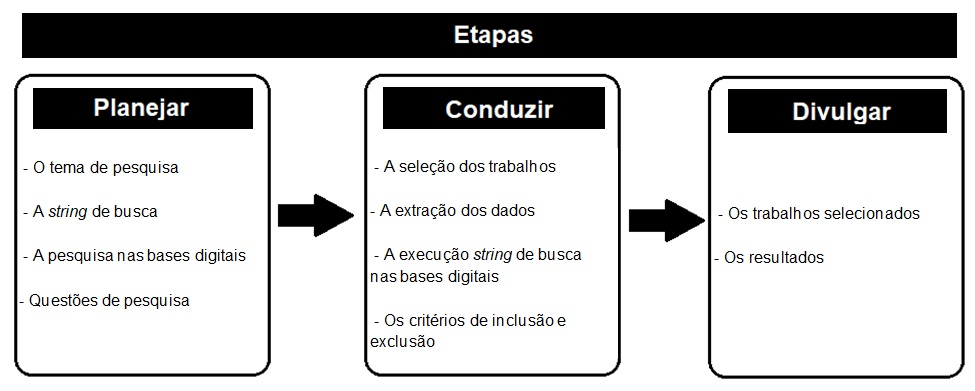
\includegraphics[width = 16cm, height=9cm]{img/etapas_RSL_final.jpg}
\caption{Etapas do mapeamento sistemático \cite{brereton2007lessons}}
\label{fig:etapasRSL}
\end{figure}

Para continuidade das atividades definidas na estratégia de busca seguindo o protocolo de pesquisa definido, a realização das consultas nas bases foi feita por meio da execução da \textit{string} de busca definida. As bases selecionadas e consultadas para a realização do mapeamento sistemático foram:
\begin{itemize}
\item \acrlong{ACM} - \url{https://dl.acm.org/}
\item \acrlong{IEEE} - \url{https://ieeexplore.ieee.org/}
\item \acrlong{SD} - \url{https://www.sciencedirect.com/}
\item \acrlong{Scps} - \url{https://www.scopus.com/}
\item \acrlong{WoS} - \url{https://www.webofknowledge.com/}
\end{itemize}

%%%%%%%%%%%%%%%%%%%%%%%%%%%%%%%%%%%%%%%%%%%%%%%%%%%%%%%%%%%%%%%%%%%%%%%%%%%%%%%%

\section{Critérios de Inclusão e Exclusão}
\label{sec:cIncExc}
Os critérios de inclusão e exclusão foram definidos para auxiliar na seleção dos trabalhos, estes critérios auxiliam na buscar por trabalhos científicos de maior relevância, e mais aderentes às questões de pesquisas definidas. 

Estes critérios foram utilizados em uma ferramenta de apoio que permitiu analisar os trabalhos parcialmente. E possibilitando incluir ou excluir da seleção os trabalhos a partir da leitura do titulo, resumo, introdução e conclusão dos trabalhos disponíveis, que foram obtidos durante a pesquisa nas bases de dados digitais.    

Os critérios de inclusão \textbf{(CI)} utilizados na seleção dos trabalhos foram:

\begin{description}

\item[CI1)] Estudo sobre monitoramento de serviços distribuídos;
\item[CI2)] Estudo sobre monitoramento de serviços em barramentos \acrshort{SOA};
\item[CI3)] Estudo sobre monitoramento de \textit{web services} pelo Protocolo \acrshort{SNMP}.
\end{description}

Os critérios de exclusão \textbf{(CE)} utilizados na seleção dos trabalhos foram:

\begin{description}
\item[CE1)] Artigos publicados com baixa relevância definidos pela pontuação de \textit{Score}\footnote{\textit{Pontuação fornecida pela ferramenta \acrshort{StArt}\textsuperscript{\textregistered}.Baixa relevância definida por \textit{Score} < 5}};
\item[CE2)] Artigos publicados como \textit{Short Paper};
\item[CE3)] Artigos publicados sem referencia com a área de Tecnologia da Informação.
\item[CE4)]Artigos cujo foco não seja monitoramento de serviços distribuídos, ou o monitoramento por Protocolo \acrshort{SNMP}, monitoramento em barramentos \acrshort{SOA}, ou monitoramento de \textit{web services};
\end{description}


%%%%%%%%%%%%%%%%%%%%%%%%%%%%%%%%%%%%%%%%%%%%%%%%%%%%%%%%%%%%%%%%%%%%%%%%%%%%%%%%

\section{Extração dos Dados}
A atividade de extração e seleção dos trabalhos foi dividida e realizada em quatro fases, a primeira fase foi a busca automática nas bases de dados digitais com a execução da \textit{string} de busca descrita na seção \ref{sec:stringbusca}, conforme o protocolo definido para busca de trabalhos científicos aderentes ao tema abordado. A segunda fase foi a realização de uma pesquisa com intenção de encontrar uma ferramenta que possibilite o registro e o gerenciamento dos trabalhos buscados, a terceira fase foi a seleção de forma manual para refinar a escolha dos trabalhos relacionados ao tema, e a quarta foi a leitura dos trabalhos seguindo os itens definidos no protocolo para extração das informações dos trabalhos selecionados. 

Durante a realização da extração dos dados por meio da execução da \textit{string} de busca em cada base obteve-se vários tipos de informações sobre os dados buscados, como por exemplo, o ano da publicação do trabalho, os locais de realização dos eventos, o \acrshort{DOI} dos trabalhos publicados, além do  expressivo número de trabalhos que uma base retornou e o número significativo que outra retornou, após a consulta realizada nas bases digitais.

\subsubsection{Fase 1}
Nessa fase foi realizada a busca dos trabalhos científicos nas bases digitais \acrlong{ACM}, \acrlong{IEEE}, \acrlong{SD}, \acrlong{Scps} e \acrlong{WoS}. Os trabalhos retornados foram obtidos por meio da utilização da \textit{string} de busca descrita na seção \ref{sec:stringbusca}, que após a execução da \textit{string} como meio de filtragem para obtenção dos trabalhos em cada base, obteve-se o retorno dos trabalhos relacionados a partir das palavras ou palavras-chave definidas na \textit{string} de busca. 

A busca nas bases de dados foi possível por causa da definição das palavras e textos registrados na \textit{string} de busca, ocasionando o refinamento por meio de filtragem de busca dos trabalhos, totalizando o número de 3.227 trabalhos publicados, que foram retornados após a pesquisa, conforme o registro na tabela \ref{tabelaresultaddos}.

\begin{table}[H]
\centering
\caption{Trabalhos retornados por base de dados digitais}
\label{tabelaresultaddos}
    \begin{tabular}{|c|c|}
        \hline
        \multicolumn{2}{|c|}{\textbf{Fase 1}} \\ \hline
        \textbf{\begin{tabular}[c]{@{}c@{}}Base de dados\end{tabular}} & \textbf{\begin{tabular}[c]{@{}c@{}}Total\end{tabular}} \\ \hline
        \acrlong{ACM}  & 86 \\ \hline
        \acrlong{IEEE}  & 68 \\ \hline
         \acrlong{SD} & 2492 \\ \hline
         \acrlong{Scps} & 515 \\ \hline
         \acrlong{WoS} & 66 \\ \hline
    \end{tabular}
\end{table}

\subsubsection{Fase 2} Após a conclusão da fase 1, que foi a realização da busca dos trabalhos nas bases científicas foi detectada a necessidade de utilização de uma ferramenta que possibilitasse um melhor controle e gerenciamento dos trabalhos científicos que foram retornados das bases. 

A necessidade surgiu por causa do grande volume de trabalhos retornados, e que durante a realização do processo de extração poderia ocasionar a perda do conhecimento ou confusão no entendimento do problema, devido a não organização dos dados obtidos pela leitura dos trabalhos. A ideia foi identificar uma ferramenta capaz de auxiliar no registro de informações obtidas na extração de trabalhos buscados. Nesse seguimento, a escolha de uma ferramenta para auxiliar no processo metodológico para na extração de dados, foi necessária e a ferramenta selecionada para execução do trabalho foi o \acrshort{StArt}\textsuperscript{\textregistered}.  

\subsubsection{Fase 3} Após a filtragem e extração dos trabalhos das bases de dados científicas, e a seleção da ferramenta de apoio para o auxílio no processo de extração dos dados, foi feita a exportação dos metadados dos trabalhos retornados de cada base digital em formato BibTex\textsuperscript{\textregistered}, como afirma o autor Chomsky \cite{chomsky1969linguistica}, após a exportação desses dados foi realizada a importação desses dados na ferramenta \acrshort{StArt}\textsuperscript{\textregistered}. 

A ferramenta possui duas etapa de funcionamento, uma para planejar e outra para executar. Na etapa de planejamento é possível a criar de um protocolo de revisão. Este protocolo é composto por um formulário onde é possível preencher: o objetivo, questões de pesquisa (principais e secundárias), palavras-chave, assim como os critérios de inclusão e exclusão. Neste mapeamento sistemático, o objetivo é a verificação de mecanismos de monitoramento em barramento de serviços distribuídos. Na etapa de execução é possível a organização dos trabalhos por base cientifica, a seleção dos trabalhos e a extração dos dados dos trabalhos científicos. Neste trabalho, a importação foi organizada por base científica digital. 

Após a importação e organização dos trabalhos por base, ferramenta sugere um \textit{score} de maior valor para os trabalhos com maior relevância aos itens definidos no protocolo de revisão, e um \textit{score} de menor valor para os trabalhos com menor relevância em referência ao protocolo definido. O \textit{score} gerado pela ferramenta, e relacionado aos trabalhos inicia em zero, que é o valor mínimo de pontuação até quarenta e um, que foi a pontuação máxima gerada após a associação do protocolo de pesquisa com os trabalhos importados. 

A partir da indicação do \textit{score} de menor valor e a verificação dos critérios de exclusão, 3.176 trabalhos foram excluídos do mapeamento sistemático, para esta exclusão foram retirados os trabalhos com \textit{score} menor que cinco. A exclusão dos trabalhos com a verificação dos critérios de exclusão, durou aproximadamente cinco semanas. 

Após a realizar a exclusão dos trabalhos de menor relevância para este trabalho, o próximo passo foi realizar a execução dos critérios de inclusão e exclusão, a fim de identificar os trabalhos com maior aderência os tema de pesquisa. 

Durante a leitura dos títulos e resumos, ou a leitura dos títulos e introduções, ou a leitura dos títulos, resumos e conclusões dos trabalhos importados, foram verificados os critérios de inclusão e exclusão para seleção dos trabalhos, com os tópicos de inclusão e exclusão descritos na seção \ref{sec:cIncExc}. 

De acordo com Petersen \textit{et al.} \cite{petersen2008systematic}, a execução desse método, visa minimizar a leitura completa de trabalhos que necessariamente não tratam do assunto. Com a utilização e verificação dos critérios de inclusão e exclusão nos trabalhos, por meio da leitura dos títulos e resumos, ou a leitura dos títulos e introduções, ou a leitura dos títulos, resumos e conclusões dos trabalhos, foi possível selecionar os trabalhos mais aderente ao tema do trabalho para leitura totalizando 51 trabalhos selecionados. A figura \ref{fig:fase3Criterios} representa a execução dos critérios para identificar os trabalhos.

\begin{figure}[H]
\centering
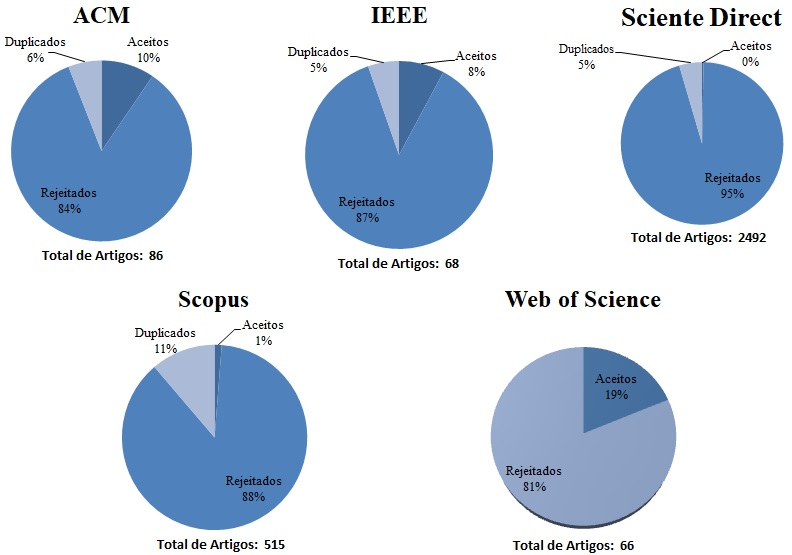
\includegraphics[width = 14cm, height=10cm]{img/Classificacao_FASE_3_CI_e_CE.jpg}
\caption{Resultado da Fase 3 classificação (CI e CE) em porcentagem.}
\label{fig:fase3Criterios}
\end{figure}

\subsubsection{Fase 4} Após a realização da classificação dos trabalhos científicos metodologicamente permitiu-se a utilização dos critérios de inclusão e exclusão obtendo o total de 51 trabalhos selecionados. Na etapa de execução, é possível além de avaliar os \textit{scores} dos trabalhos com a possibilidade para classificar, na ferramenta, o status de seleção dos trabalhos (Aceito, Rejeitado e Duplicado) e a prioridade de leitura (Muito alta, alta, baixa e muito baixa). 

Neste trabalho, após a leitura dos títulos e resumos, ou a leitura dos títulos e introduções, ou a leitura dos títulos, resumos e conclusões dos 51 trabalhos selecionados, foi realizada a classificação de aceitação e prioridade de leitura. Nesse seguimento, foram obtidos 29 trabalhos aceitos, mas com a indicação para prioridade de leitura baixa, por apresentarem pouca aderência e relevância ao tema proposto, e 22 trabalhos aceitos com indicação de prioridade de leitura alta, por possuírem, maior relevância e aderência ao tema, para a leitura completa dos trabalhos.   

Após a classificação foi iniciada a 4º fase, com 22 trabalhos aceitos e com prioridade de leitura alta, que possibilitou a observação mais aprofundada nos trabalhos com maior aderência ao tema. 

A partir da leitura completa dos trabalhos, a ferramenta \acrshort{StArt}\textsuperscript{\textregistered} foi utilizada para continuidade do mapeamento sistemático, onde nessa fase foram incluídos nos formulários da ferramenta, atributos definidos no protocolo de pesquisa, e especificamente registrados como "campos para extração dos dados", que possibilitou o registro de informações, com a leitura completa dos trabalhos, o  que permitiu a posteriori à avaliação dos trabalhos por meio de uma a análise empírica. 

As devidas anotações e classificações de cada trabalho foi registrada na ferramenta, o que permitiu catalogar o trabalho para facilitar a recuperação dos pontos mais importantes, de uma forma mais rápida e precisa, assim como identificar os trabalhos mais relevantes e aderentes às questões de pesquisa. Após a leitura, e ainda a realização de registros e análise dos trabalhos obteve-se uma leitura e entendimento dos 22 trabalhos extraídos e selecionados dos 51 trabalhos que foram selecionados nessa fase. 

\vspace{30mm}

\begin{longtable}{c|c|c|c|c|c|c|}
\caption{Trabalhos excluídos, incluídos, rejeitados e selecionados.}
\label{tab:fase-revisao-literatura}\\
\cline{2-7}
 & \multicolumn{6}{c|}{Base de Dados} \\ \cline{2-7} 
\endfirsthead
%
\endhead
%
 & Critério & \acrshort{ACM} & \acrlong{IEEE} & \acrlong{SD} & \acrlong{Scps} & \acrlong{WoS} \\ \hline
\multicolumn{1}{|c|}{Fase 2} & Busca & 86 & 68 & 2492 & 515 & 66 \\ \hline
\multicolumn{1}{|c|}{\multirow{5}{*}{Fase 3}} & CE1 & 37 & 18 & 1529 & 259 & 21 \\ \cline{2-7} 
\multicolumn{1}{|c|}{} & CE2 & 18 & 15 & 460 & 156 & 15 \\ \cline{2-7} 
\multicolumn{1}{|c|}{} & CE3 & 14 & 9 & 299 & 61 & 14 \\ \cline{2-7} 
\multicolumn{1}{|c|}{} & CE4 & 9 & 7 & 198 & 33 & 4 \\ \cline{2-7} 
\multicolumn{1}{|c|}{} & CI1, CI2, CI3 & 8 & 19 & 6 & 6 & 12 \\ \hline
\multicolumn{1}{|c|}{\multirow{2}{*}{Fase 4}} & Rejeição & 0 & 18 & 6 & 4 & 1 \\ \cline{2-7} 
\multicolumn{1}{|c|}{} & Seleção & 8 & 1 & 0 & 2 & 11 \\ \hline
\end{longtable}

Os 51 trabalhos selecionados estão na tabela \ref{tab:51-artigos}, e os 22 trabalhos selecionados para  realização da extração contribuíram para o mapeamento sistemático do trabalho, estão da tabela \ref{tab:tabelaresultadosAnalise}. A revisão é fundamental para auxiliar e fundamentar o conhecimento a fim subsidiar as respostas das questões de pesquisa. 

\begin{longtable}{|c|l|l|}
\caption{Trabalhos selecionados.}
\label{tab:51-artigos}\\
\hline
ID & \multicolumn{1}{c|}{Título} & \multicolumn{1}{c|}{Referęncia} \\ \hline
\endfirsthead
%
\endhead
%
1 & \begin{tabular}[c]{@{}l@{}}Service Oriented \\ Architecture-based \\ Framework for \\ WBAN-enabled \\ Patient Monitoring \\ System\end{tabular} & \begin{tabular}[c]{@{}l@{}}Abousharkh, Maha and Mouftah, \\ Hussein \cite{abousharkh2011service}.\end{tabular} \\ \hline
2 & \begin{tabular}[c]{@{}l@{}}An Investigation of Monitoring \\ Configurations\end{tabular} & \begin{tabular}[c]{@{}l@{}}Abdu, Hasina and Lutfiyya, Hanan L.\\  and Bauer, Michael A \cite{abdu1995investigation}.\end{tabular} \\ \hline
3 & \begin{tabular}[c]{@{}l@{}}Monitoring, Accounting and \\ Automated Decision Support for \\ the Alice Experiment Based on \\ the MonALISA Framework\end{tabular} & \begin{tabular}[c]{@{}l@{}}Cirstoiu, Catalin C. and Grigoras, \\ Costin C. and Betev, \\ Latchezar L. and Costan, \\ Alexandru A. and Legrand, \\ Iosif Charles \cite{cirstoiu2007monitoring}. \end{tabular} \\ \hline
4 & \begin{tabular}[c]{@{}l@{}}Scaling a Monitoring \\ Infrastructure \\ for the Akamai Network\end{tabular} & \begin{tabular}[c]{@{}l@{}}Repantis, Thomas and Cohen, \\ Jeff and Smith, Scott and Wein, Joel \cite{repantis2010scaling}.\end{tabular} \\ \hline
5 & \begin{tabular}[c]{@{}l@{}}Implementing and Operating an \\ Internet Scale Distributed \\ Application Using Service \\ Oriented Architecture Principles\\  and Cloud Computing \\ Infrastructure\end{tabular} & Sedayao, Jeff \cite{sedayao2008implementing}. \\ \hline
6 & \begin{tabular}[c]{@{}l@{}}A Scalable SNMP-based \\ Distibuted Monitoring System \\ for Heterogeneous Network \\ Computing\end{tabular} & \begin{tabular}[c]{@{}l@{}}Subramanyan, Rajesh and \\ Miguel-Alonso, José and \\ Fortes, José A. B. \cite{subramanyan2000scalable}.\end{tabular} \\ \hline
7 & \begin{tabular}[c]{@{}l@{}}Monitoring Distributed \\ Systems\end{tabular} & \begin{tabular}[c]{@{}l@{}}Joyce, Jeffrey and Lomow, \\ Greg and Slind, Konrad and Unger, \\ Brian \cite{joyce1987monitoring}.\end{tabular} \\ \hline
8 & \begin{tabular}[c]{@{}l@{}}Monitoring Overhead in \\ Distributed Systems: \\ Visualization and Estimation \\ Techniques\end{tabular} & \begin{tabular}[c]{@{}l@{}}Abdu, Hasina and Lutfiyya, \\ Hanan and Bauer, Michael A.\cite{abdu1996monitoring}.\end{tabular} \\ \hline
9 & \begin{tabular}[c]{@{}l@{}}Improvements to online \\ distributed monitoring \\ systems\end{tabular} & \begin{tabular}[c]{@{}l@{}}Wang, Bo and Song, Ying and \\ Sun, Yuzhong and Liu, Jun \cite{wang2016improvements}.\end{tabular} \\ \hline
10 & \begin{tabular}[c]{@{}l@{}}A Formal Engineering \\ Approach for Control and \\ Monitoring Systems in \\ a Service-Oriented \\ Environment\end{tabular} & \begin{tabular}[c]{@{}l@{}}Nagorny, Kevin and Harrison, \\ Robert and Colombo, Armando \\ Walter andKreutz, Gerhard \cite{nagorny2013formal}.\end{tabular} \\ \hline
11 & \begin{tabular}[c]{@{}l@{}}Personal Health Service \\ Framework\end{tabular} & Ghorbani, Shirin and Du, Weichang \cite{ghorbani2013personal}.\\ \hline
12 & \begin{tabular}[c]{@{}l@{}}JMonitor: A monitoring tool \\ for distributed systems\end{tabular} & \begin{tabular}[c]{@{}l@{}}Penteado, Mauricio G. and \\ Trevelin, Luis Carlos \cite{penteado2012jmonitor}.\end{tabular} \\ \hline
13 & \begin{tabular}[c]{@{}l@{}}Agent Technology in \\ Monitoring Systems\end{tabular} & Patrut, Bogdan and Tomozei, Cosmin \cite{puatruct2010agent}. \\ \hline
14 & \begin{tabular}[c]{@{}l@{}}Cryptanalysis of the application \\ secure alternative to SNMP \\ (APSSNMP)\end{tabular} & Phan, Raphael C. -W. \cite{phan2009cryptanalysis}. \\ \hline
15 & \begin{tabular}[c]{@{}l@{}}Profiling Node Conditions of \\ Distributed System with \\ Sequential PatternMining\end{tabular} & Hirate, Yu and Yamana, Hayato\cite{hirate2009profiling}. \\ \hline
16 & \begin{tabular}[c]{@{}l@{}}SeNsIM-Web: a Service Based \\ Architecture for Sensor \\ Networks Integration\end{tabular} & \begin{tabular}[c]{@{}l@{}}Casola, Valentina and Gaglione, \\ Andrea and Mazzeo, Antonino \cite{casola2009sensim}.\end{tabular} \\ \hline
17 & \begin{tabular}[c]{@{}l@{}}A SOA-based information \\ management model for \\ Next-Generation Network\end{tabular} & \begin{tabular}[c]{@{}l@{}}Kotsopoulos, Konstantinos and \\ Lei, Pouwan and Hu, Yim Fun \cite{kotsopoulos2008soa}.\end{tabular} \\ \hline
18 & \begin{tabular}[c]{@{}l@{}}A Flexible Monitoring and \\ Notification System for \\ Distributed Resources\end{tabular} & Smith, Garry and Baker, Mark \cite{smith2008flexible}. \\ \hline
19 & \begin{tabular}[c]{@{}l@{}}Design and implementation \\ of the SNMP agents for \\ remote monitoring \\ andcontrol via UML and \\ Petri nets\end{tabular} & Lee, JS and Hsu, PL \cite{lee2004design}. \\ \hline
20 & \begin{tabular}[c]{@{}l@{}}Distributed mobile \\ communication base \\ station diagnosis and \\ monitoringusing \\ multi-agents\end{tabular} & \begin{tabular}[c]{@{}l@{}}Feng, JQ and Buse, DP and \\ Wu, QH and Fitch, J.  \cite{feng2002distributed}.\end{tabular} \\ \hline
21 & \begin{tabular}[c]{@{}l@{}}An authentication and \\ authorization solution \\ supporting SOA-based \\ distributed systems\end{tabular} & \begin{tabular}[c]{@{}l@{}}P. Qi-rui and W. Cheng and W. Jing and \\ L. Jun and L. \\ Qing and S. Bei-en \cite{qi2010authentication}.\end{tabular} \\ \hline
22 & \begin{tabular}[c]{@{}l@{}}Scalable Agentless \\ Cloud Network Monitoring\end{tabular} & M. Brattstrom and P. Morreale \cite{brattstrom2017scalable}.\\ \hline
23 & \begin{tabular}[c]{@{}l@{}}Implementation of secure \\ customized monitoring tool for\\ adapative distributed systems\end{tabular} & \begin{tabular}[c]{@{}l@{}}M. Kotari and N. N. \\ Chiplunkar and H. R. Nagesh \cite{kotari2014implementation}.\end{tabular} \\ \hline
24 & \begin{tabular}[c]{@{}l@{}}Multi-layer SOA \\ implementation \\ pattern with service \\ and data proxies for \\ distributed \\ data-intensive \\ application \\ system\end{tabular} & Takdir and A. I. Kistijantoro \cite{kistijantoro2014multi}. \\ \hline
25 & \begin{tabular}[c]{@{}l@{}}ABMOM for cross-platform \\ communication in SOA \\ systems\end{tabular} & \begin{tabular}[c]{@{}l@{}}N. M. Ibrahim and M. F. Hassan and \\ M. H. Abdullah \cite{ibrahim2013abmom}.\end{tabular} \\ \hline
26 & \begin{tabular}[c]{@{}l@{}}Reliable ESB and Distributed \\ Transactional Memory for SOA\end{tabular} & S. Yong and R. Yi-Zhi \cite{yong2012reliable}. \\ \hline
27 & \begin{tabular}[c]{@{}l@{}}Technologies for SOA-based \\ distributed large scale process \\ monitoring and control systems\end{tabular} & \begin{tabular}[c]{@{}l@{}}F. Jammes and B. Bony and \\ P. Nappey and A. W. \\ Colombo and J. Delsing and \\ J. Eliasson and R. Kyusakov\\ and S. Karnouskos and \\ P. Stluka and M. Till \cite{jammes2012technologies}.\end{tabular} \\ \hline
28 & \begin{tabular}[c]{@{}l@{}}Agent-based intelligent \\ monitoring in large-scale \\ continuous material transport\end{tabular} & Y. Pang and G. Lodewijks \cite{pang2012agent}. \\ \hline
29 & Web Services Open Test Suites & N. El Ioini \cite{el2011web}. \\ \hline
30 & \begin{tabular}[c]{@{}l@{}}Researching and Designing the \\ Architecture of \\ E-government Based on SOA\end{tabular} & P. Yan and J. Guo \cite{yan2010researching}. \\ \hline
31 & \begin{tabular}[c]{@{}l@{}}Towards Role-Based \\ Self-healing\\ in Autonomous \\ Monitoring Systems\end{tabular} & \begin{tabular}[c]{@{}l@{}}W. Funika and P. Pegiel and \\ M. Bubak and J. Kitowski \cite{funika2010towards}.\end{tabular} \\ \hline
32 & \begin{tabular}[c]{@{}l@{}}Modeling Service Oriented \\ Architectures of Mobile \\ Applications by Extending \\ SoaML with Ambients\end{tabular} & N. Ali and M. A. Babar \cite{ali2009modeling}.\\ \hline
33 & \begin{tabular}[c]{@{}l@{}}Research on Multi-tier \\ Distributed Systems Based \\ on AOP and Web Services\end{tabular} & J. Zhang and F. Meng and G. Liu \cite{zhang2009research}. \\ \hline
34 & \begin{tabular}[c]{@{}l@{}}Research on SOA-Based \\ Applications Based on \\ AOP and Web Services\end{tabular} & J. Zhang and F. Meng and G. Liu \cite{zhang2008research}. \\ \hline
35 & \begin{tabular}[c]{@{}l@{}}Monitoring distributed \\ embedded systems\end{tabular} & R. Ford \cite{ford1990monitoring}. \\ \hline
36 & Monitoring distributed systems & M. Mansouri-Samani and M. Sloman \cite{mansouri1993monitoring}. \\ \hline
37 & \begin{tabular}[c]{@{}l@{}}The dark side of SOA testing: \\ Towards testing contemporary \\ SOAs based on criticality \\ metrics\end{tabular} & \begin{tabular}[c]{@{}l@{}}P. Leitner and S. Schulte and \\ S. Dustdar and I. Pill and M. \\ Schulz and F. Wotawa \cite{leitner2013dark}.\end{tabular} \\ \hline
38 & \begin{tabular}[c]{@{}l@{}}Leveraging Service Oriented \\ Architecture: A case study \\ for ocean energy information \\ management\end{tabular} & A. Bosnjak and S. Huang and J. J. Mulcahy \cite{bosnjak2011leveraging}. \\ \hline
39 & \begin{tabular}[c]{@{}l@{}}A managerial community of \\ Web Services for management \\ of communities of Web Services\end{tabular} & \begin{tabular}[c]{@{}l@{}}A. Benharref and M. A. Serhani and \\ S. Bouktif and J. Bentahar \cite{benharref2010managerial}.\end{tabular} \\ \hline
40 & \begin{tabular}[c]{@{}l@{}}Decision guidance models \\ for microservice monitoring\end{tabular} & Haselbock, S. and Weinreich, R. \cite{haselbock2017decision}. \\ \hline
41 & \begin{tabular}[c]{@{}l@{}}Building the monitoring \\ systems for complex \\ distributed systems: \\ Problems \& solutions\end{tabular} & \begin{tabular}[c]{@{}l@{}}Korableva, O. and Kalimullina, O. \\ and Kurbanova, E. \cite{korableva2017building}.\end{tabular} \\ \hline
42 & \begin{tabular}[c]{@{}l@{}}Pattern detection model \\ for monitoring distributed \\ systems\end{tabular} & Dinu, C.-M. and Pop, F. and Cristea, V. \cite{dinu2011pattern}. \\ \hline
43 & \begin{tabular}[c]{@{}l@{}}Dynamic agent based \\ monitoring mechanism for \\ web services\end{tabular} & Wen, J. and Zhao, L. and He, P. \cite{wen2011dynamic}. \\ \hline
44 & \begin{tabular}[c]{@{}l@{}}A performance study of \\ monitoring and information \\ services for distributed \\ systems\end{tabular} & Zhang, X. and Freschl, J.L. and Schopf, J.M. \cite{zhang2003performance}. \\ \hline
45 & \begin{tabular}[c]{@{}l@{}}HiFi: a new monitoring \\ architecture for distributed \\ systems management\end{tabular} & \begin{tabular}[c]{@{}l@{}}Al-Shaer, Ehab and Abdel-Wahab, \\ Hussein and Maly, Kurt \cite{al1999hifi}.\end{tabular} \\ \hline
46 & \begin{tabular}[c]{@{}l@{}}Goal-driven adaptive \\ monitoring of SOA \\ systems\end{tabular} & Marek Psiuk and Krzysztof Zielinski \cite{psiuk2015goal}. \\ \hline
47 & \begin{tabular}[c]{@{}l@{}}On heuristics for \\ optimal configuration of \\ hierarchical distributed \\ monitoring systems\end{tabular} & \begin{tabular}[c]{@{}l@{}}Jiannong Cao and Kang Zhang and \\ Olivier de Vel \cite{cao1998heuristics}.\end{tabular} \\ \hline
48 & \begin{tabular}[c]{@{}l@{}}What Can Web \\ Services Bring to \\ Integrated Management?\end{tabular} & Aiko, Pras and Jean-Philippe Martin-Flatin \cite{pras2008can}. \\ \hline
49 & \begin{tabular}[c]{@{}l@{}}Transformer Fleet \\ Monitoring\end{tabular} & \begin{tabular}[c]{@{}l@{}}Jaković, Tihomir, Ivan \\ Murat, Filip Klarić and\\  Samir Keitoue \cite{jakovic2017transformer}.\end{tabular} \\ \hline
50 & \begin{tabular}[c]{@{}l@{}}Model-based monitoring \\ and policy enforcement \\ of services\end{tabular} & \begin{tabular}[c]{@{}l@{}}Xiaoying Bai and Yongli Liu and \\ Lijun Wang and Peide Zhong \cite{bai2009model}.\end{tabular} \\ \hline
51 & \begin{tabular}[c]{@{}l@{}}Web Service Diagnoser \\ Model for managing faults \\ in web services\end{tabular} & K. Jayashree and Sheila Anand \cite{jayashree2013web}. \\ \hline
\end{longtable}


%%%%%%%%%%%%%%%%%%%%
\begin{longtable}{|c|l|l|}
\caption{Trabalhos selecionados para leitura completa}
\label{tab:tabelaresultadosAnalise}\\
\hline
ID & \multicolumn{1}{c|}{Título} & \multicolumn{1}{c|}{Referência} \\ \hline
\endfirsthead
%
\endhead
%
1 & \begin{tabular}[c]{@{}l@{}}Service Oriented\\ Architecture-based\\ Framework for WBAN-\\ enabled Patient\\ Monitoring System\end{tabular} & \begin{tabular}[c]{@{}l@{}}Abousharkh, Maha and Mouftah, \\ Hussein. \cite{abousharkh2011service}.\end{tabular} \\ \hline
2 & \begin{tabular}[c]{@{}l@{}}An Investigation of\\ Monitoring Configurations\end{tabular} & \begin{tabular}[c]{@{}l@{}}Abdu, Hasina and Lutfiyya, Hanan L. \cite{abdu1995investigation}.\end{tabular} \\ \hline
3 & \begin{tabular}[c]{@{}l@{}}Monitoring, Accounting\\ and Automated\\ Decision Support for the\\ Alice Experiment\\ Based on the MonALISA\\ Framework\end{tabular} & \begin{tabular}[c]{@{}l@{}}Cirstoiu, Catalin C. and Grigoras, \\ Costin C. and Betev, Latchezar L. \\ and Costan, Alexandru A. and Legrand,\\ Iosif Charles. \cite{cirstoiu2007monitoring}.\end{tabular} \\ \hline
4 & \begin{tabular}[c]{@{}l@{}}Scaling a\\ Monitoring Infrastructure\\ for the Akamai Network\end{tabular} & \begin{tabular}[c]{@{}l@{}}Repantis, Thomas and\\ Cohen, Jeff and\\ Smith, Scott and Wein,\\ Joel. \cite{repantis2010scaling}.\end{tabular} \\ \hline
5 & \begin{tabular}[c]{@{}l@{}}Implementing and\\ Operating an Internet\\ Scale Distributed\\ Application Using\\ Service Oriented\\ Architecture Principles\\ and Cloud\\ Computing\\ Infrastructure\end{tabular} & Sedayao, Jeff. \cite{sedayao2008implementing}. \\ \hline
6 & \begin{tabular}[c]{@{}l@{}}Scalable SNMP-\\ based Distibuted\\ Monitoring System\\ for Heterogeneous\\ Network Computing\end{tabular} & \begin{tabular}[c]{@{}l@{}}Subramanyan, Rajesh\\ and Miguel-Alonso, José\\ and Fortes, José A. \cite{subramanyan2000scalable}.\end{tabular} \\ \hline
7 & \begin{tabular}[c]{@{}l@{}}Monitoring Distributed\\ Systems\end{tabular} & \begin{tabular}[c]{@{}l@{}}Joyce, Jeffrey and\\ Lomow, Greg\\ and Slind, Konrad and\\ Unger, Brian. \cite{joyce1987monitoring}.\end{tabular} \\ \hline
8 & \begin{tabular}[c]{@{}l@{}}Dynamic agent based\\ monitoring mechanism\\ for web services \end{tabular} & Wen, J. and Zhao, L. and He, P. \cite{Junhao} \\ \hline
9 & \begin{tabular}[c]{@{}l@{}}Monitoring Overhead\\ in Distributed\\ Systems: Visualization\\ and Estimation\\ Techniques\end{tabular} & \begin{tabular}[c]{@{}l@{}}Abdu, Hasina and\\ Lutfiyya,\\ Hanan and Bauer,\\ Michael A. \cite{abdu1996monitoring}.\end{tabular} \\ \hline
10 & \begin{tabular}[c]{@{}l@{}}Improvements\\ to online distributed\\ monitoring systems\end{tabular} & \begin{tabular}[c]{@{}l@{}}Wang, Bo and\\ Song, Ying and\\ Sun, Yuzhong and\\ Liu, Jun. \cite{wang2016improvements}\end{tabular} \\ \hline
11 & \begin{tabular}[c]{@{}l@{}}Scalable Agentless\\ Cloud Network Monitoring \end{tabular} & \begin{tabular}[c]{@{}l@{}}M. Brattstrom and P. Morreale \cite{Brattstrom_7987194}.\end{tabular} \\ \hline
12 & \begin{tabular}[c]{@{}l@{}}Personal Health\\ Service Framework\end{tabular} & \begin{tabular}[c]{@{}l@{}}Ghorbani, Shirin\\ and Du, Weichang. \cite{ghorbani2013personal}.\end{tabular} \\ \hline
13 & \begin{tabular}[c]{@{}l@{}}JMonitor: A\\ monitoring tool for\\ distributed systems\end{tabular} & \begin{tabular}[c]{@{}l@{}}Penteado, Mauricio\\ G. and Trevelin, Luis\\ Carlos. \cite{penteado2012jmonitor}.\end{tabular} \\ \hline
14 & \begin{tabular}[c]{@{}l@{}}Agent\\ Technology in\\ Monitoring Systems\end{tabular} & \begin{tabular}[c]{@{}l@{}}Patrut, Bogdan\\ and Tomozei,\\ Cosmin. \cite{puatruct2010agent}.\end{tabular} \\ \hline
15 & \begin{tabular}[c]{@{}l@{}}Cryptanalysis\\ of the application\\ secure alternative\\ to SNMP (APSSNMP)\end{tabular} & \begin{tabular}[c]{@{}l@{}}Phan, Raphael\\ C. -W. \cite{phan2009cryptanalysis}.\end{tabular} \\ \hline
16 & \begin{tabular}[c]{@{}l@{}}Profiling Node\\ Conditions of Distributed\\ System\\ with Sequential\\ PatternMining\end{tabular} & \begin{tabular}[c]{@{}l@{}}Hirate, Yu and\\ Yamana,\\ Hayato. \cite{hirate2009profiling}.\end{tabular} \\ \hline
17 & \begin{tabular}[c]{@{}l@{}}SeNsIM-Web: a Service\\ Based Architecture for\\ Sensor Networks\\ Integration\end{tabular} & \begin{tabular}[c]{@{}l@{}}Casola, Valentina\\ and Gaglione, Andrea\\ and Mazzeo, Antonino. \cite{casola2009sensim}.\end{tabular} \\ \hline
18 & \begin{tabular}[c]{@{}l@{}}A SOA-based\\ information\\ management model\\ for Next-Generation\\ Network\end{tabular} & \begin{tabular}[c]{@{}l@{}}Kotsopoulos,\\ Konstantinos and Lei,\\ Pouwan and Hu, Yim\\ Fun. \cite{kotsopoulos2008soa}.\end{tabular} \\ \hline
19 & \begin{tabular}[c]{@{}l@{}}A Flexible\\ Monitoring and\\ Notification System\\ for Distributed\\ Resources\end{tabular} & \begin{tabular}[c]{@{}l@{}}Smith, Garry\\ and Baker,\\ Mark. \cite{smith2008flexible}.\end{tabular} \\ \hline
20 & \begin{tabular}[c]{@{}l@{}}Design\\ and implementation\\ of the SNMP agents\\ for remote monitoring\\ andcontrol via UML\\ and Petri nets\end{tabular} & \begin{tabular}[c]{@{}l@{}}Lee, JS and\\ Hsu, PL. \cite{lee2004design}.\end{tabular} \\ \hline
21 & \begin{tabular}[c]{@{}l@{}}Distributed mobile\\ communication\\ base station diagnosis\\ and monitoringusing\\ multi-agents\end{tabular} & \begin{tabular}[c]{@{}l@{}}Feng, JQ and\\ Buse, DP and\\ Wu, QH and Fitch, J. \cite{feng2002distributed}.\end{tabular} \\ \hline
22 & \begin{tabular}[c]{@{}l@{}}Building the monitoring \\ systems for complex distributed \\ systems: \\ Problems \& solutions \end{tabular} & \begin{tabular}[c]{@{}l@{}}Korableva, O. and Kalimullina, O. and \\ Kurbanova, E.. \cite{korableva2017building}.\end{tabular} \\ \hline
\end{longtable}

%%%%%%%%%%%%%%%%%%%%%%%%%%%%%%%%%%%%%%%%%%%%%%%%%%%%%%%%%%%%%%%%%%%%%%%%%%%%%%%%

\section{Resultados}
Após a realização da pesquisa dos trabalhos, com a maior relevância e maior aderência ao tema de pesquisa nas bases digitais, a seleção e extração dos trabalhos para leitura, nesta seção por meio da utilização do mapeamento sistemático. 

Será possível responder às questões de pesquisa descritas na seção \ref{questoes1e2} de forma fundamentada pelos trabalhos científicos obtidos por meio de resumos referentes às questões. 

As leituras dos trabalhos ampliaram o conhecimento sobre o tema, e permitiram a identificação e apresentação dos seguintes itens, para utilizá-los como base para execução do projeto, são eles:
\begin{itemize}
\item Monitoramento de sistemas distribuídos
\item \textit{Web services}
\item Agentes de monitoramento
\item Protocolo \acrshort{SNMP}
\item Armazenamento das Informações monitoradas
\item Desempenho
\end{itemize}

\subsubsection{QP1) Quais os estudos primários existentes na literatura que discutem os mecanismos de monitoramento que são aplicados a sistemas distribuídos?}

\subsubsection{Monitoramento de Sistemas Distribuídos}
Na seleção dos trabalhos realizou-se uma pesquisa que foi identificada a necessidade do monitoramento de sistemas distribuídos, devido à grande quantidade de  aplicações, dispositivos e \textit{web services} em funcionamento, e que normalmente não possuem acompanhamento durante o seu funcionamento. 

O autor Penteado \cite{penteado2012jmonitor}, descreve sobre a importância das ferramentas de monitoramento possuírem padrões, para a transferência de dados aos Agentes de monitoramento. 

No trabalho descrito por Cirstoiu \textit{et al.} \cite{cirstoiu2007monitoring},  sobre o monitoramento de sistemas distribuídos e da utilização das API's para comunicação de aplicativos e a preocupação com o baixo acoplamento dessas ferramentas. 

Em outro trabalho,  este descrito por Joyce \textit{et al.}\cite{joyce1987monitoring}, sobre a importância do monitoramento de sistemas distribuídos, e a utilização de testes de programas para verificação dos sistemas monitorados. 

No entanto o autor Abdu \textit{et al.} \cite{abdu1995investigation}, descreve o quanto é complexo o gerenciamento do monitoramento de sistemas distribuídos, sendo necessário a utilização de técnicas e métricas para obtenção dos resultados coletados, por conta da grande quantidade de informações geradas pelo monitoramento.  

\subsubsection{\textit{Web Services}}

Os autores Abousharkh \textit{et al.}, Casola \textit{et al.} e Ghorbani \textit{et al.} \cite{abousharkh2011service,casola2009sensim,ghorbani2013personal}, apresentam em seus trabalhos, como a flexibilidade e agilidade no desenvolvimento de \textit{web services}, podem trazer resultados imediatos paras aplicações, suas características que facilitam a integração dos serviços e sistemas, e como é fácil a integração de ambientes com os padrões da Indústria e protocolos como SOAP e HTTP, porém a facilidade abre uma preocupação referente à segurança das aplicações, principalmente no que tange a integridade e confidencialidade dos dados.  Também relatam sobre desafios como implementar uma solução que seja flexível, escalável e interoperável.  

\subsubsection{Agentes de Monitoramento}

Agentes de monitoramento podem ser um dispositivo ou um software, esses podem ser utilizados para realizar a comunicação ou notificação do monitoramento de outros dispositivos ou sistemas distribuídos. 

O autor Smith \textit{et al.} \cite{smith2008flexible}, explica sobre a utilização e comparação de ferramentas (\textit{plugins}) que funcionam como agentes de monitoramento de sistemas distribuídos e também da arquitetura definida para o gerenciamento e acompanhamento. 

O autor Pătruţ \textit{et al.} \cite{puatruct2010agent}, relata sobre o experimento com informações metacognitivas que proporcionaram 12 definições para identificação de agentes inteligentes, propostas para definição de um agente ou Super agente, e como eles podem monitorar sistemas para realização de comunicação homem-máquina.

O autor Feng \textit{et al.} \cite{feng2002distributed} discorre em seu trabalho sobre a importância da realização de monitoramento por agentes, devido o grande numero de serviços disponíveis, e que por vários motivos que podem sofrer alguma interferir no funcionamento, e projeta a implementação de serviços com multiagentes para fornecer desempenho na transmissão de informações do monitoramento pelos agentes.

\subsubsection{Protocolo SNMP}
\label{snmpDescription}

O autor Lee \textit{et al.} \cite{lee2004design}, descreve sobre a qualidade do Protocolo \acrshort{SNMP}, seu principais componentes e utilização da estação de gestão, agente de gestão, base de informações de gestão e o protocolo de gestão e suas vantagens. 

Apesar  de  seu  nome,  \acrlong{SNMP},  o  \acrshort{SNMP}  é  um protocolo  relativamente  complexo  para  implementar.  Também,  o  \acrshort{SNMP}  não  é  um protocolo muito eficiente. Os autores Phan e Subramanyan \textit{et al.} \cite{phan2009cryptanalysis,subramanyan2000scalable} também relatam sobre alguns pontos fracos, como a vulnerabilidade presente no SNMPv1, desempenho e falta de escalabilidade.

\subsubsection{QP2) Quais são as principais características relativas ao monitoramento de sistemas distribuídos mencionadas na literatura?}

\subsubsection{Armazenamento das Informações Monitoradas}

O Monitoramento dos sistemas distribuídos quando implementados geram informações durante a execução, essas informações são importantes para acompanhar o funcionamento de sistemas distribuídos e \textit{web services}. O autor Repantis \textit{et al.} \cite{repantis2010scaling}, explica sobre a importância da coleta dessas informações e a coleta em larga escala utilizando instruções e comandos \textit{SQL}. Porém devido ao grande número de sistemas distribuídos monitorados e a grande quantidade de informações geradas por meio do monitoramento, os autores Abdu \textit{et al.} e Hirate \textit{et al.} \cite{abdu1996monitoring,hirate2009profiling} apresentam as técnicas para mensurar a sobrecarga gerada pela quantidade de informações e padrões de mineração dos dados armazenados.  

\subsubsection{Desempenho}

O autor Wang \cite{wang2016improvements}, apresenta algoritmos de compactação de dados, para realização de transferência dos dados de modo otimizado, devido à grande quantidade de informações geradas durante o monitoramento dos sistemas distribuídos. Nesse trabalho foram realizados vários testes, incluído conversão de formatos, como por exemplo, arquivos XML. 

O autor Sedayao \cite{sedayao2008implementing}, descreve como a falta de experiência para implementar \textit{web services} para realização de monitoramento, impactaram diretamente no desempenho da aplicação, e como adquiriram experiência para a implementação de forma correta dos serviços, tornando a aplicação robusta, e altamente distribuída. 

Já o autor Kotsopoulos \textit{et al.} \cite{kotsopoulos2008soa}, explica o motivo da não utilização do protocolo \acrshort{SNMP}, por conta de algumas limitações, como por exemplo, a escalabilidade e eficiência. 

\subsubsection{Escalabilidade}

A escalabilidade de sistemas distribuídos está entre as principais características técnicas de funcionamento, ela busca disponibilizar o acesso às aplicações mesmo com o aumento gradativo de usuários. O autor Brattstrom \textit{et al.} \cite{Brattstrom_7987194}, descreve que o sistema de computação distribuída deve ser dimensionado para o uso de um grande número de recursos de computação, a tendência é aumentar devido a grande evolução cibernética. No entanto, os sistemas devem escalar de modo que não atrapalhe o desempenho dos sistema, a escalabilidade é encarada com um desafio. 

Nesse seguimento a autora Korableva \textit{et al.} \cite{korableva2017building}, relata a preocupação com a utilização de sistemas de monitoramento, que possam ser implementados de forma sistema integrada, escalável e fácil de usar, em seu trabalho descreve um método para alcançar esse objetivo em seu experimento. O autor Wen \textit{et al.} \cite{Junhao}, descreve a medida que o número de serviços à ser monitorado aumenta, o sistema tem impacto negativo na flexibilidade e escalabilidade, principalmente no tempo de resposta. A capacidade de um sistema pode ser aprimorada de maneira direta, e utiliza uma solução implementada que trabalha dinamicamente, para oferecer suporte a uma maior carga de informações durante a realização do monitoramento, sem sofrer degradação perceptível no desempenho do tempo de resposta. 

\vspace{10mm}
\noindent

Com o mapeamento sistemático, foi possível identificar os trabalhos com maior relevância e aderência ao tema deste trabalho. Pode-se perceber pontos, positivos e negativos sobre os itens definidos para pesquisa, o monitoramento de sistemas distribuídos, \textit{Web services}, agentes de monitoramento, o  Protocolo \acrshort{SNMP}, sobre o armazenamento das informações monitoradas e a preocupação como desempenho Verificar os trabalhos, também contribuíram para identificar os principais desafios relacionados à este trabalho.


\section{Síntese do Capítulo}

Este capítulo apresentou a execução do mapeamento sistemático para identificar nos trabalhos científicos, dados e informações relacionadas ao monitoramento de sistemas, ao protocolo de monitoramento \acrshort{SNMP} e ferramentas de monitoramento, dessa maneira conseguir ir possibilitando a fundamentação para implementação do projeto de monitoramento dos serviços do barramento Erlangms, com a utilização do protocolo \acrshort{SNMP} para integração com ferramentas de monitoramento. O protocolo \acrshort{SNMP} foi identificado como solução para implementação do projeto, visto que o \acrshort{CPD} atualmente já utiliza, pois possui ferramentas de monitoramento que realizam o monitoramento de \textit{softwares} e ativos de rede, por meio do protocolo. 

%%%%%%%%%%%%%%%%%%%%%%%%%%%%%%%%%%%%%%%%%%%%%%%%%%%%%%%%%%%%%%%%%%%%%%%%%%%%%%%%%%%%%